%# -*- coding: utf-8-unix -*-
%%==================================================
%% chapter01.tex for SJTU Master Thesis
%%==================================================

%\bibliographystyle{sjtu2}%[此处用于每章都生产参考文献]
\chapter{系统设计}
\label{chap:systemdesign}
DOBBS是为了适应大规模IaaS云的底层存储,利用对象存储对非结构化数据VMDI进行大量优化,并且在WHOBBS的基础上解决了其性能缺陷。本章我将介绍DOBBS的
系统架构设计以及各模块设计。

\section{DOBBS架构介绍}
所谓混合存储系统,就是将SSD与HDD共同组合而成的存储系统。DOBBS的系统设计是基于Ceph实现的,而Ceph的文件实际是存储在对象存储设备中的(Objects 
Storage Device)。为了提升DOBBS系统的高扩展性,我们借用了Ceph存储池(Storage Pool)的概念。存储池实际是部分对象存储设备的逻辑集合,一个存储池
可以包含多个对象存储设备,而对象存储设备是挂载在物理存储介质上的。因此对于DOBBS,我们有两种类型的对象存储设备,分别是SSD对象存储设备和HDD对象存储设备。
之后,我们将部分SSD对象存储设备和部分HDD对象存储设备共同组织成一个混合存储池(Hybrid Storage Pool)。混合存储池中的对象存储设备是可以由用户配置的,
通过这样的组织,DOBBS的底层存储集群可以简单高效地扩展。一般性的,每个混合存储池都至少包括一个SSD对象存储设备和至少一个HDD对象存储设备。


\begin{figure}[!htp]
    \centering
    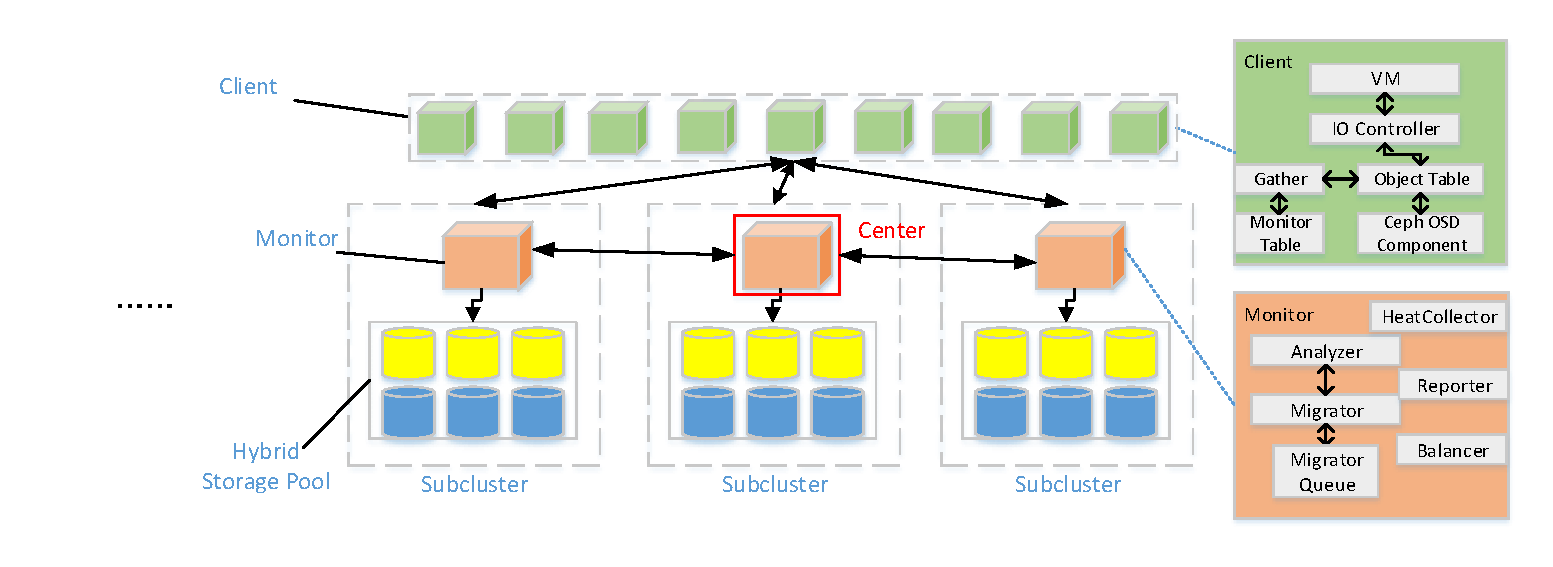
\includegraphics[width=16cm]{example/Arch.pdf}
    \bicaption[fig:arch]{DOBBS系统架构图}{DOBBS系统架构图}{Fig}{Architecture of DOBBS}
   \end{figure}


如图\ref{fig:arch}所示为DOBBS的系统架构图。DOBBS的架构大致可以分为两层,一层是存储集群也就是混合存储池,一层是监控器(Monitor)。DOBBS包含大量
的混合存储池以及监控器。存储集群正如上文所说的,它是有大量的混合存储池组成的。为了系统的高可靠性和高性能,我们将一个监控器和一个混合存储池绑定在一起,组成一个子
集群(subcluster)。之所以要划分成子集群是因为多个Monitor如果同时管理所有的混合存储池势必会造成管理的混乱,并大大降低系统的可扩展性。引入子集群则是可以充分
提升系统的可扩展性,并使整个系统易于管理。监控器在DOBBS则是起到至关重要的作用,它的作用包括监控虚拟机的数据流信息并生成合适的迁移策略,还有检测其所在子集群的热度并向中心节点(Center)
汇报,最终执行全局热均衡迁移指令。在DOBBS中,子集群仅仅只是逻辑上的概念,虚拟机VMDI则被均匀的分布在各个子集群的混合存储池中。监控器所监控的数据流信息也仅仅是其所在
子集群对应数据的数据流信息。客户端(Client)则是虚拟机管理器(VMM)所运行的机器,它们是DOBBS所提供服务的对象,客户端在接入DOBBS之后,与底层存储系统交互并进行数
据读写。中心节点则是DOBBS的监控器集群的大脑,它的主要作用是收集每个子集群的热度信息,并保证整个系统的热均衡。关于整个系统的热均衡,在本章后续章节将会叙述。

为了系统的高内聚低耦合,我们将系统分为多个模块,模块间互相依赖并支持高效扩展。在客户端上,如果让虚拟机管理器直接访问Ceph的块存储,那么它只需要调用Ceph提供的
OSD Component接口即可,但是为了获得虚拟机的数据流信息我们VM与Ceph存储设备的交互中间增加了一层DOBBS监控组件。因为Ceph是对象存储系统,所以虚拟机访问的粒度都是
一个个对象。如图\ref{fig:arch}所示,IO Controller负责截取VM的访问请求,然后通过查询Object Table来知道对象是在哪个OSD上,这是因为在数据迁移的过程中对象被频繁迁移,
而Ceph访问对象是通过对象ID和OSD共同组合访问,因此需要一个数据结构在存储对象ID和OSD ID的映射。Gather模块类似于一个计数器,它会记录每一个单位时间间隔内的
对象的访问次数、访问类型等信息,在记录之后再定时发送给Monitor。Monitor Table则是用来维护OSD ID和子集群ID映射的,因为在DOBBS在保证整个系统热均衡的过程中需要对OSD上的数据进行跨子集群迁移,所以
可能会导致某个OSD的位置发生了改变。最终,Ceph根据VM请求的对象ID和OSD ID来和底层存储进行交互。

Monitor主要有六个模块。Analyzer模块是Monitor的大脑,它负责接收客户端传送过来的虚拟机数据流信息,然后根据内置算法来生成合适的对象迁移命令,命令产生后将迁移命令传递给
Migrator模块执行。Migrator得到迁移指令之后,进行后续的上锁等等操作,然后再将最终的指令缓存在Migrator Queue中,这个队列的长度是DOBBS所支持的最大迁移数量,这个数量
当然也是可配置的。在Monitor上还有三个独立的模块,Reporter、HeatCollector和Blancer,他们都是用来负责系统热均衡的。

DOBBS提出了两个重要的概念,局部热均衡和全局热均衡。对于局部热均衡,我们数据对象分为两类,热对象和冷对象。所谓热对象是指的那些访问频率高,短时间内会被多次访问的对象。相反,
冷对象则是指那些访问频率并不高的对象。为了充分利用SSD的性能优势,我们将热对象都放置于SSD上而将冷对象都放置于HDD上,然后动态地监测数据对象的冷热变化来在SSD和HDD之间迁移对象。
局部热均衡只是针对每个子集群内部的局部热均衡,因此每个Monitor只能保证所在子集群的局部热均衡。


如果将存储集群和Monitor分割成多个子集群,那么极有可能在某个时刻某个虚拟机产生了非常大量的VMDI请求,这样某个子集群会遭受大量的读写请求,数据也会频繁地在SSD和HDD间迁移,这个子集群的效率将会受到极大
影响。提出全局热均衡的概念就是为了消除上述情况带来的性能波动。全局热均衡针对的粒度是OSD级别的,它会动态监测每个子集群的热度,然后做出迁移指令,有别于局部热均衡的迁移,全局热均衡的迁移是将OSD的数据进
行迁移而不是在OSD进行数据对象的迁移。

\section{局部热均衡}
因为SSD相较于HDD在读写速度上都有非常大的优势,并且SSD因为并不是采用机械的方式访问数据,所以也更加节能,在现在的数据中心中是存储的主流。但是,目前的SSD价格还是十分昂贵,容量
更是十分有限。如\citen{zhang2015skewly}所介绍的,冷数据和热数据实际也是符合80/20规律的,那么将数量较少的热数据放置于SSD数量较多的冷数据放置于HDD的策略是符合SSD容量小HDD容量大
特点的。DOBBS的局部热均衡则是动态地实现了数据的放置和迁移,我们从VM对数据的访问收集数据的信息,做出迁移策略。局部热均衡在保证存储效率的同时,也让整个存储的实现更加经济。值得注意的是局部
热均衡是针对每个子集群内部的热均衡。

\subsection{VM数据流监测和分析}
Ceph是一个对象存储系统,在VMDI创建之后,Ceph会把VMDI分割成大量对象存储于OSD上\cite{weil2006ceph}。因此局部热均衡锁面向的数据流信息指的是Ceph中每个对象的数据流信息。VM数据流的产生
源头是位于Client上的虚拟机管理器,如果安装原生Ceph的逻辑,虚拟机管理器直接和Ceph的OSD访问模块交互,进行数据读取。但是,我们需要获取VM数据流信息就必须将VM与Ceph的OSD访问模块截断。
当VM请求VMDI对象时,它会先经过IO Controller的访问控制。IO Controller主要实现两个功能,一是通过对象ID查询到OSD ID,二是记录这个对象的访问次数。之所以需要通过对象ID查询OSD ID,是因为
Ceph访问数据对象是通过对象ID和OSD ID共同组合访问的,但是局部热均衡会将对象在在OSD之间频繁移动,所以需要一个数据结构记录每个对象是在哪一个OSD上。Object Table就是用来记录对象位于哪个OSD
的数据结构。IO Controller通过对象ID在Object Table中查询VM请求对象所在的OSD,然后调用Ceph OSD Component来后续的对象读写。IO Controller的第二个功能是,记录这个请求对象的访问次数和
访问类型。在DOBBS中,我们刻画对象的数据流信息通过对象ID、访问类型(随机访问或顺序访问)以及单位时间内访问次数。IO Controller将截取的对象数据流信息交给Gather模块来进行统计和整合。Gather
模块在接收到IO Controller传递过来的数据流信息之后,记录下数据流信息,然后将单位时间内的数据流信息发送给Monitor,最后再清空计数器。

当Monitor收集到了从客户端节点发送来的数据流信息之后,它开始通过数据流信息计算每个对象的热度。这里提到的热度实际是一个具象化的数值。局部热均衡实际就是通过这个热值作为依据来进行对象的迁移。
Anlyzer模块就是主要负责,对象热值的计算以及得出合适的数据放置策略。考虑到虚拟机上运行的应用程序的多变性和复杂性,用一套通用的算法来计算数据对象的热度值并不是很现实。所以,DOBBS提供了更加
开放的方式,我们提供了算法接口API,这样用户可以直接继承这个接口来适配性地使用自己的热度值计算方法。我们还提供了一个默认的计算方法,沿用了WHOBBS\cite{lingxuan2015whobbs}的计算方法。
如\ref{eq:objheat}所示,在单位时间$t$内某一个对象的热度是这样计算的。其中$sio$指的是在$t$时间内顺序读写的数量,而$rio$指的是在$t$时间内随机读写的数量。$S$和$R$是两个常数,
它们分别表示顺序读写所占的比例和随机读写所占的权重。

\begin{equation}
    \label{eq:objheat}
    CurObjHeat_t = sio_t \cdot S + rio_t \cdot R
  \end{equation}

Anlyzer在计算完每个对象权重之后就开始启动周期性轮询机制产生对象迁移指令,它内部会维护一个有序的队列,这个队列描述了每一个对象热度值和其所在的OSD编号并且是通过每个对象的热度值降序排序。DOBBS做
SSD和HDD间的数据迁移是一种贪心的策略,我们始终保证热的对象可以占满整个SSD。所以,Anlyzer会周期性轮询有序队列,从对头取出一定数量的对象,让它们放置于SSD上。在系统刚刚加载时,我们默认所有对象
都位于HDD。Ceph默认的对象大小是64MB,所以根据SSD大小来决定多少个对象放置于SSD上。例如,128GB的SSD最多可以放置2000个对象,那么每次将队列头的2000个对象置于SSD,如果对象原来所在的位置是HDD,
则产生HDD到SSD的迁移指令。相反,如果遍历到对象是队列2000个以后,并且在SSD上的,则产生SSD到HDD的迁移指令。

\subsection{对象迁移}
Anlyzer在产生迁移指令之后,Migrator则负责实际的对象迁移工作。Migrator首先会检查,当前的SSD是否已满,如果SSD已满则会终止掉当前的迁移请求。接下来,Migator将每一条迁移指令缓存下来,并存入迁移队列
Migrat Queue中。如果Migrator同时让多个对象进行迁移,那么对整个系统的性能将会是灾难性的影响。因为对象的传输将会大大占用网络带宽,并且DOBBS为了维护迁移过程中对象的一致性,需要频繁地对Client的对象
上锁和解锁,那么同时大量对象迁移将会影响VM的性能。所以,Migrate Queue保证了系统同时最大迁移数量,如果系统中已经有部分对象在做迁移,那么后续的迁移指令需要等待之前的迁移完成之后才可以执行。

\section{全局热均衡}
